%Seperator
%Seperator
%Seperator
%Seperator
%Seperator
\section{Airfoil Computational Analysis}
\begin{comment}
\end{comment}
$$R = \frac{\rho U L}{\mu}$$
Taking density of air to be $\rho=1.225\,kgm^{-3}$, dynamic viscosity $\mu=1.81\times10^{-5}\,kgm^{-1}s^{-1}$. 
Our stall speed was prescribed by the requirements to be around $V_{stall} = 4.572\,ms^{-1}$. 
Our chord length is predicted to be around $0.12\,m$ at the smallest part of the wing so to be safe, let us try to simulate for chord length of around $0.05\,m$. The \texttt{Python} script below is used to compute the Reynold's number,
%$$R = (rho*U*L)/mu$$
\lstinputlisting[language=Python]{Programming/R_Num.py}
$$$$
The results of running the algorithm for the stall speed and minimum chord length gives the lower bound Reynold's number that the \texttt{xflr} simulations ought to be run at,
\begin{lstlisting}
>>> R_Num(4.572, 0.05)
15471.546961325967
\end{lstlisting}
$$$$
Running the algorithm for the same stall speed but at the predicted maximum chord length of around $0.4\,m$ gives us the upper bound Reynold's number that the \texttt{xflr} simulations should be run at,
\begin{lstlisting}
>>> R_Num(4.572, 0.4)
123772.37569060773
\end{lstlisting}
$$$$
For extra insurance, let us run our \texttt{xflr} analysis on the range of .
\begin{equation}10000 \leq R_{e} \leq 150000 \label{Re req}\end{equation}


%Seperator
%Seperator
%Seperator
%Seperator
%Seperator
\section{Algorithm Development}
\begin{comment}
\end{comment}
Below describes the theoretical algorithmic flow:
\begin{enumerate}
\item Given an airfoil, we are going to run for a series of Reynold's number ranges prescribed based on equation $\ref{Re req}$. 
\item For each of those Reynold's number, we are going to run simulations for a range of angles of attack. The range of the angles of attack is going to be high enough such that we can figure out the stall angle of attack and the corresponding maximum lift coefficient.
\item Now each airfoil for differing Reynold's number is going to have different stall angles and different corresponding maximum lift coefficient. Stall is a separation effect and it is a very bad regime to fly in. Therefore, we want to choose flight regimes without stall. This is just the limit of the airfoil.
\item This means that for a given airfoil, amongst all the different maximum lift coefficient due to Reynod's number variation, we will choose the minimum $c_{L,max}$.
\item We will also compute the average maximum lift coefficients for a given airfoil amongst its differing Reynold's number ranges justto compare that the minimum $c_{L,max}$ is not due to results that have failed to converge.
\end{enumerate}
The simulation will require extensive file manipulations such as renaming, moving files around, and requires the interaction of many programs. Therefore, the language of choice for this simulation would be the \texttt{Bash}. We are going to present a series of \texttt{Bash} scripts that is used to automate testing and work. There will be a few data analysis section and for that we decided to use \texttt{Python} due to its ease and extensive data-related libraries.
%Seperator
\\~\\This is how the algorithm's directory tree is structured. All of the related \texttt{Bash} and \texttt{Python} scripts will be placed in only a single directory. Within that directory where all of the source code resides, there will be just a single directory that contains all of the Airfoil-specific data and this directory is creatively named \texttt{Airfoil\_Data}. Let us first go through how the files are prepared.

%Seperator
%Seperator
%Seperator
%Seperator
\subsection{Setup\_Airfoil\_Selection\_Algorithm} \label{setup script}
\begin{comment}
\end{comment}
The \texttt{Bash} script below is used to fetch all of the necessary airfoil data from the web databases and store the airfoil coordinates in individual directories. These individual directories will then be placed inside the data directory named \texttt{Airfoil\_Data}. Let us examine the various utilities called from within this shell script, 
\lstinputlisting[language=Bash]{Programming/Setup_Airfoil_Selection_Algorithm}
$$$$
Note to run the set-up shell script, it is very easy, just call the following command. Everything else should be handled for you after calling that command.
\begin{lstlisting}
./Setup_Airfoil_Selection_Algorithm
\end{lstlisting}

%Seperator
%Seperator
%Seperator
%Seperator
\subsection{Fetch\_Airfoils}
\begin{comment}
\end{comment}
Ok, so the first utility called by the script shown in section $\ref{setup script}$ is \texttt{Fetch\_Airfoils}. I mentioned about fetching data automatically from web-servers right? Well this is exactly what the script does! \texttt{wget} is a common \texttt{Linux} utility that allows the download of a certain file from the web. So the way \texttt{wget} is used in this instance is like this:
\begin{lstlisting}[language=Bash]
wget WEB_ADDRESS -O NAME_FILE
\end{lstlisting}
For different airfoils, we just change the argument \texttt{WEB\_ADDRESS} with where we believe the airfoil coordinate file is located in the internet. We would also want to give the downloaded file a good name we like. For that, we change the argument \texttt{NAME\_FILE}. Anyways, this is not a tutorial on how to use \texttt{wget}, more details can be found in its official site documentation. For now, the script below fetches all of the airfoi cordinates in selig format from different web-addresses and renames them.
\lstinputlisting[language=Bash]{Programming/Fetch_Airfoils}

%Seperator
%Seperator
%Seperator
%Seperator
\subsection{Produce\_Airfoil\_List}
\begin{comment}
\end{comment}
So after running \texttt{Fetch\_Airfoils} we are going to have a bunch of files named \texttt{Eppler\_Airfoil\_whatever.dat}, \texttt{Another\_Random\_Airfoil.dat} and so on for all of the airfoils we listed in the script above. So now it would be convenient if we have a file containing just the names of the airfoils. This file would then be used in naming the various directories that the airfoil coordinate files would be placed in.
\lstinputlisting[language=Bash]{Programming/Produce_Airfoil_List}

%Seperator
%Seperator
%Seperator
%Seperator
\subsection{Make\_Airfoil\_Directories}
\begin{comment}
\end{comment}
This \texttt{Bash} script takes an input file as an argument and then goes through the contents of that file, making new directories corresponding to each airfoil inside the given input file and then putting the airfoil coordinate data into the newly-created directory.
\lstinputlisting[language=Bash]{Programming/Make_Airfoil_Directories}

%Seperator
%Seperator
%Seperator
%Seperator
\subsection{Move\_Airfoil\_Directories}
\begin{comment}
\end{comment}
This \texttt{Bash} script has a simple task, move all the directories found inside a file list to a new location that is given by the second input argument. This is used to move all of the newly created directories corresponding to each airfoil into a directory named \texttt{Airfoil\_Data}. 
\lstinputlisting[language=Bash]{Programming/Move_Airfoil_Directories}


%Seperator
%Seperator
%Seperator
%Seperator
\subsection{Multi\_Airfoil\_Analysis}
\begin{comment}
\end{comment}
This is the next \texttt{Bash} script that needs to be explained. This \texttt{Bash} script is the allows us to perform analysis on multiple airfoils in one single run. After we have done all of the initial setup described in section $\ref{setup script}$, we can run the airfoil analysis by invoking the command,
\begin{lstlisting}
./Multi_Airfoil_Analysis Airfoil_List.txt
\end{lstlisting}
wherein \texttt{Airfoil\_List.txt} is a text file containing all of the airfoil names mentioned previously. \texttt{Multi\_Airfoil\_Analysis}  depends on a lot of other scripts. So the script will run all the Reynold's Number simulations and stall conditions for each listed airfoil, collect all of the data from all of the listed airfoils and output the summary in a file named \texttt{Raw\_Multi\_Airfoil\_Analysis.tex}. 
\lstinputlisting[language=Bash]{Programming/Multi_Airfoil_Analysis}

%Seperator
%Seperator
%Seperator
%Seperator
\subsection{Ave\_CL\_Max.py}
\begin{comment}
\end{comment}
We are counting on the \texttt{Single\_Airfoil\_Re\_Analysis} to basically generate a file corresponding to each airfoil containing the various Reynold's numbers the particular airfoil was tested at as well as the maximum lift coefficient. This \texttt{Python} script operates on that file, gets rid of all of the invalidated data where stall conditions were not met or poor convergence was obtained and then using the valid data points, figure out the average maximum lift coefficient and the smallest lift coefficient for that airfoil across all of its Reynold's number ranges. 
\lstinputlisting[language=Python]{Programming/Ave_CL_Max.py}

%Seperator
%Seperator
%Seperator
%Seperator
\subsection{Single\_Airfoil\_Re\_Analysis}
\begin{comment}
\end{comment}
Now that we have explained the way multiple airfoils are considered, we need to examine how individual airfoils are considered at a time. This \texttt{Bash} script is responsible for calling a few functionalities which would be explained in more detail.
\lstinputlisting[language=Bash]{Programming/Single_Airfoil_Re_Analysis}

%Seperator
%Seperator
%Seperator
%Seperator
\subsection{Gen\_Input\_File}
\begin{comment}
\end{comment}
We have decided to interface with \texttt{Xfoil} directly using the terminal. To interface with \texttt{Xfoil} we need to give it command instructions. Now the script shown below generates the \texttt{XFoil} specific instructions needed to run simulations at a desired Reynold's number and a range of angle of attack.
\lstinputlisting[language=Bash]{Programming/Gen_Input_File}

%Seperator
%Seperator
%Seperator
%Seperator
\subsection{Comment\_Out}
\begin{comment}
\end{comment}
After \texttt{Xfoil} has completed running, we need to comment the first few lines with \texttt{\#} so that \texttt{Python} can easily read in and analyze the data using \texttt{numpy}. This script does that. It adds the character \texttt{\#} into the first $12$ lines of a specified file.
\lstinputlisting[language=Bash]{Programming/Comment_Out}

%Seperator
%Seperator
%Seperator
%Seperator
\subsection{Read\_Polar.py}
\begin{comment}
\end{comment}
This is another \texttt{Python} script that operates on a single file that \texttt{Xfoil} generates. \texttt{XFoil} is going to generate lift coefficients and angles of attack at a particular Reynold's number. This \texttt{Python} script checks if the simulation run in \texttt{xfoil} has indicated the presence of a stall and what is the maximum lift coefficient at that stall angle.
\lstinputlisting[language=Python]{Programming/Read_Polar.py}

%Seperator
%Seperator
%Seperator
%Seperator
\subsection{Plot\_Airfoil\_Geom.py}
\begin{comment}
\end{comment}
Scripts which are named starting with \texttt{Plot} are basically just diagnostic tools. These are scripts used only to examine the data and make give a clearer picture of the behaviour of these airfoil simulations. This particular script plots the airfoil geometry. It might be useful to examine if the panels are sufficiently high resolution or if further refinemenet is necessary.
\lstinputlisting[language=Python]{Programming/Plot_Airfoil_Geom.py}
$$$$
An example of using the script is shown below,
\begin{lstlisting}
./Plot_Airfoil_Geom.py Airfoil_Data/S1223/S1223.dat
\end{lstlisting}
The command above would plot the \texttt{S1223} airfoil coordinate files.

%Seperator
%Seperator
%Seperator
%Seperator
\subsection{Plot\_CLMax\_Re.py}
\begin{comment}
\end{comment}
Scripts which are named starting with \texttt{Plot} are basically just diagnostic tools. We know that for different Reynold's Numbers, the maximum lift coefficient is going to vary. This \texttt{Python} script plots the relationship between the maximum lift coefficient as a function of Reynold's number for just one particular airfoil. It is very useful to tell anomalous results occuring in which Reynold's Number cases.
\lstinputlisting[language=Python]{Programming/Plot_CLMax_Re.py}
$$$$
An example of using the script above to plot the maximum lift coefficient with Reynold's Number for a particular airfoil,
\begin{lstlisting}
./Plot_CLMax_Re.py Airfoil_Data/Eppler_E_423/Eppler_E_423_Multi_Re.tex
\end{lstlisting}
The command above would plot the maximum lift coefficient vs Reynold's Number for the \texttt{Eppler\_E\_423} airfoil.

%Seperator
%Seperator
%Seperator
%Seperator
\subsection{Plot\_CL\_Alpha.py}
\begin{comment}
\end{comment}
Scripts which are named starting with \texttt{Plot} are basically just diagnostic tools. This particular script plots lift coefficient as a function of angle of attack $\alpha$. Now this script only works for a single airfoil for a single Reynold's number case.
\lstinputlisting[language=Python]{Programming/Plot_CL_Alpha.py}
$$$$
An example of using the script above to plot the lift coefficient as a function of angle of attack for a particular airfoil at a particular Reynold's number is shown below,
\begin{lstlisting}
./Plot_CL_Alpha.py Airfoil_Data/Church_Hollinger/Church_Hollinger_Output_RE_30000.tex 
\end{lstlisting}
The command above would plot the lift coefficient vs angle of attack for the \texttt{Church Hollinger} airfoil at a Reynold's Number of $30000$.

%Seperator
%Seperator
%Seperator
%Seperator
%Seperator
\section{Results of Computational Analysis}
\begin{comment}
\end{comment}
From the $10$ initial airfoils chosen, here are the tabulated results,
\lstinputlisting{Programming/Raw_Multi_Airfoil_Analysis.tex}
$$$$
As one can see, there are several convergence issues with \texttt{Xfoil} for some of the airfoils. We decided that $2$ good candidates for further testing would be the \texttt{Selig 1223} airfoil and the \texttt{Eppler E 423} airfoils. Both airfoils are highly cambered and have a substantial leading edge thickness, just like what we wanted.

\begin{figure}[H]\centering
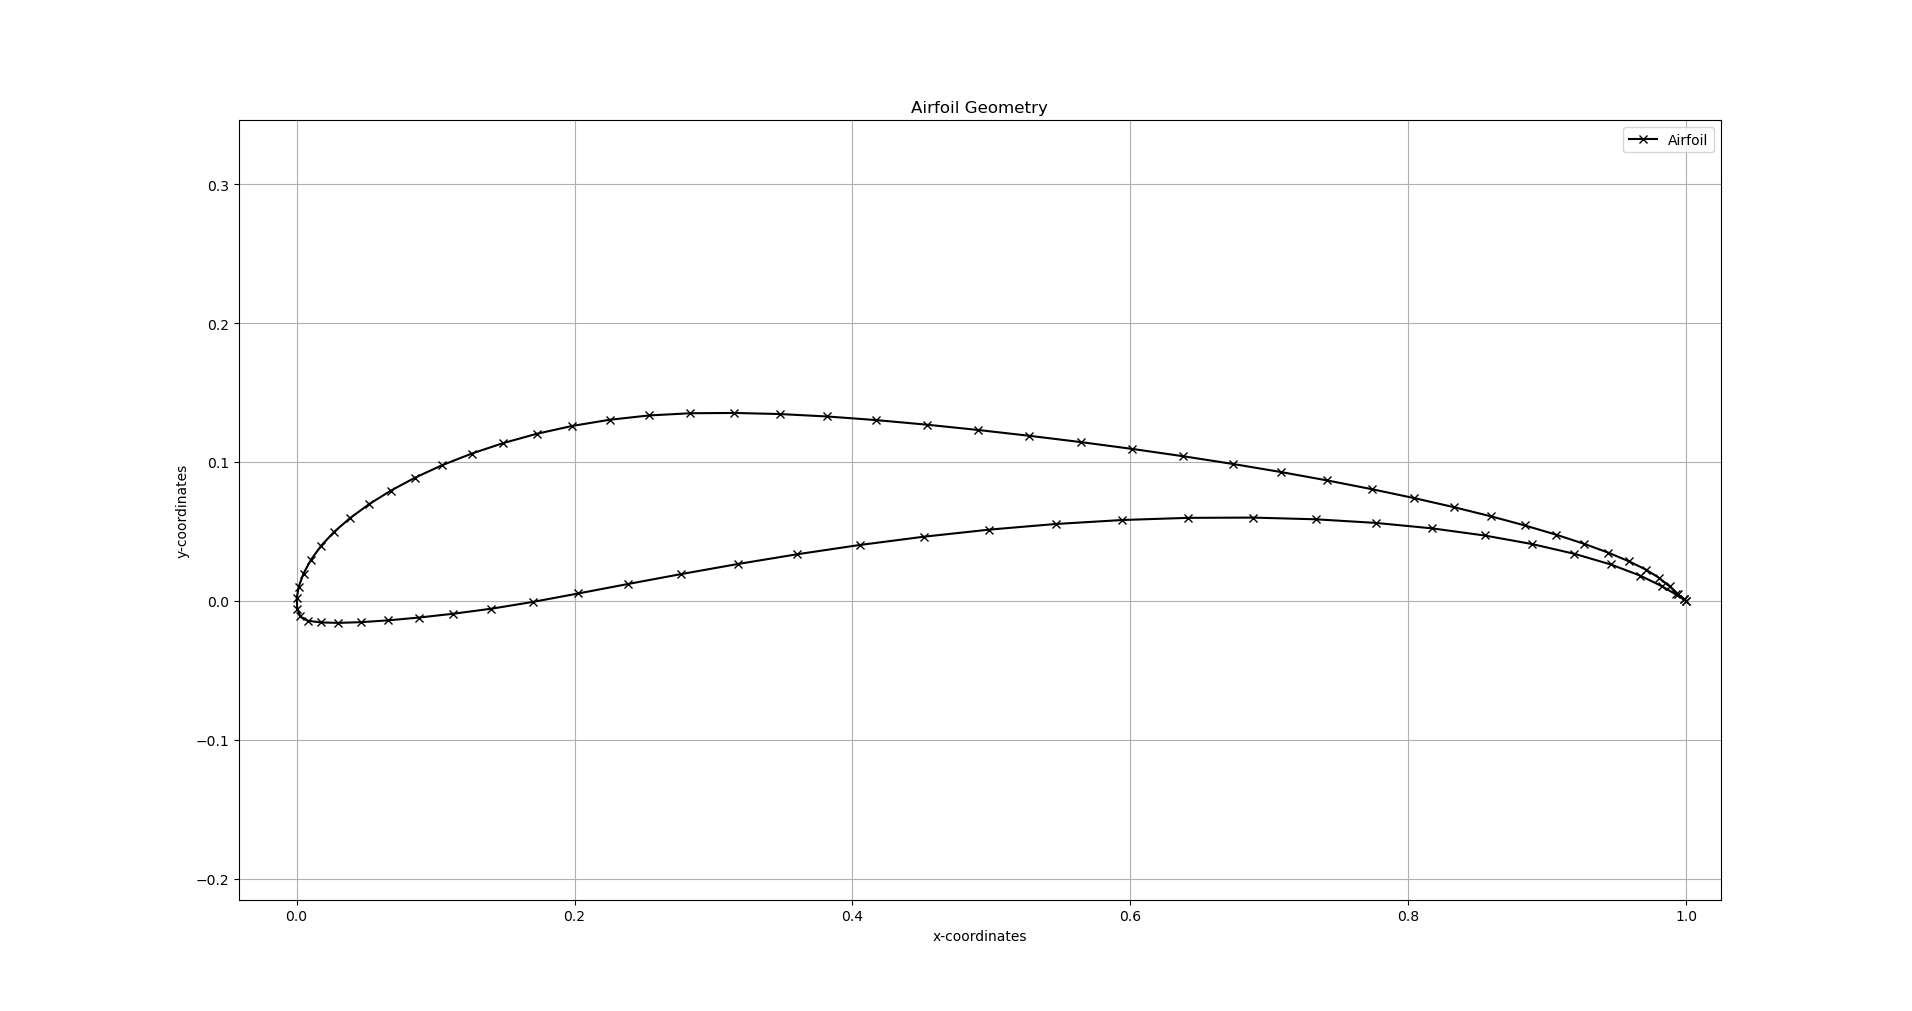
\includegraphics[scale=\size]{Content/Images/Selig_1223_Sketch.png}
\caption{Representation of the Selig 1223 Airfoil}
\label{Selig_Sketch}
\end{figure}
\begin{figure}[H]\centering
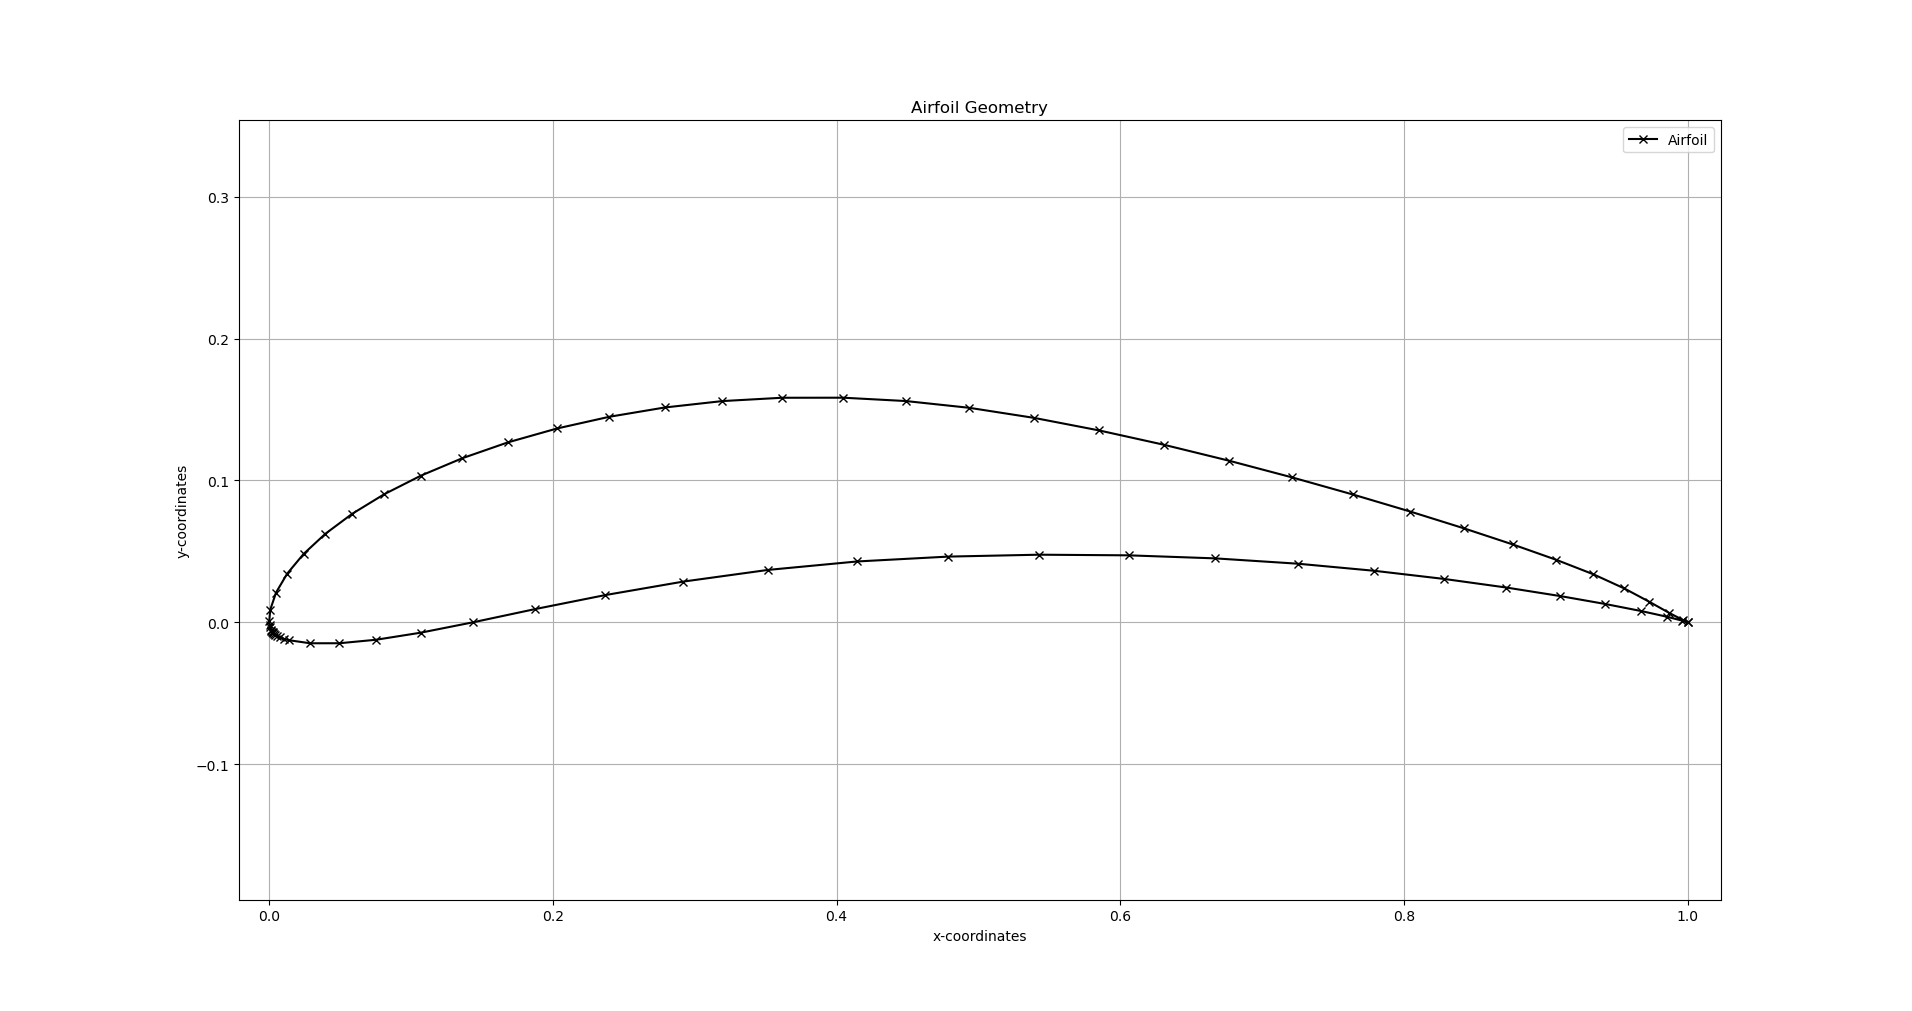
\includegraphics[scale=\size]{Content/Images/Eppler_E_423.png}
\caption{Representation of the Eppler E 423 Airfoil}
\label{Eppler_Sketch}
\end{figure}



